\chapter[Computational Model]{Computational Model}
\label{chap:computational_model}

\lettrine{C}{alculating} changes to be performed based on user behavior is the challenge in question of this chapter.
The model presented here suggests a computational description of the convergence (or divergence) phenomenon, which aims to match the process the phonetic internal representation undergoes during a conversation.

\pagebreak

\todo[inline]{change (all?) \enquote{convergence} to \enquote{accommodation}}

\section{From \acs{hhi} to \acs{hci}}
\label{sec:from_hhi_to_hci}

The experiments presented in \cref{part:experiments} show humans' accommodative behaviors in different \ac{hhi} and \ac{hci} settings.
Complementary to that, \cref{subsec:accommodation_levels} discusses ways to represent various level of accommodative behaviors in computers.
Since behavioral changes, as explained by \ac{cat} (see \cref{sec:communication_accommodation_theory}), happen naturally and often unconsciously in \ac{hhi}, it is not trivial to transfer them to computers, which need defined rules and numeric representation to process.
These can be achieved by applying some measuring technique appropriate for each feature, like formant values for vowel quality or frequency for \ac{f0}.
Creating rules for different behaviors, however, cannot be directly constructed, due to the nature of this intuitive phenomenon, but rather inferred from observed \ac{hhi} data.
For example, The results of the study described in \cref{chap:shadowing_experiment_with_natural_and_synthetic_voices} reveal high degree of variation across participants.
\todo{take a slides about individual differences to show some differences either here or at the mentioned section}
While this is expected, further examination of these variations uncovers some general properties that can be taken as a ground for characterizing the different changes.
The link between the measured raw values and systematic rules should be a machine-applicable equivalence of the convergence process in humans.
Such parallelisms would need to model, for instance, the way humans percept the convergence-prone sounds, how they interact with previous instances and the current internal state of the sound in question, and the cognitive process of the the phonetic changes.
Therefore, such a model should include the perception of the phonetic features, representation of the change in state of each feature in memory, and the realization of the changes during a conversation.
As these parts of the process are, by definition, dependent on each other, the computational model presented in \cref{sec:pipeline_representation} depicts them as a pipeline where each of its steps stand for an action performed, unconsciously, by a human speaker.

\section{Pipeline representation}
\label{sec:pipeline_representation}

As convergence happens automatically and seamlessly in human interlocutors' cognition, it is hard to say what are the exact steps this process comprises.
Some key properties stand out when examining many occurrences in different interactions.
The pipeline presented here aims to capture these properties and offer a defined process of describing the changes.
The advantages of representing this process as a pipeline (as opposed to, e.g., a one-step, end-to-end conversion) is that each part in the process can be interpreted and controlled separately (see \cref{subsec:computational_model,fig:adaptation_module_pipeline}).
This enables combining different methods and implementations while keeping the steps independent of each other.
Therefore, only the \emph{order} of execution is important, which does not introduces any limitation, as long as it is consistent.
This modular structure makes the execution of specific steps more flexible, like introducing different ways to calculate accommodation.
Substituting specific steps' techniques grants the freedom to experiment with different methods without losing the core principles of the accommodation process.
For example, substituting the calculation method in the \textit{update} step or replacing it with a statistical method (see \cref{chap:statistical_model})
\putref{add mentions for ML/DL models chapters/sections if there are any}
will of course influence the output of this step, but will not alter its role in the pipeline's overall logic.
Note that although only speech-related features are discussed here, this pipeline could be used in principle for describing changes in other type of features or modalities, like lexical choices, linguistic complexity, eye gaze, emotional state, etc.

In short, the proposed pipeline representation consists of the following five main steps, which are explained in detail in \crefrange{subsec:detect}{subsec:assign}:
%
\begin{itemize}[topsep=0cm, itemsep=-.1cm, wide=0cm, leftmargin=!, labelwidth=\widthof{\textbf{update}}]
	\item[\textbf{detect}] hear and identify a feature that can be changed, corresponding to a human's ear's ability to notice such variations;
	
	\item[\textbf{filter}] decide whether the encountered feature's instance appears in a way that can trigger change, capturing the inherent detection of phonological context and rules in the language;
	
	\item[\textbf{collect}] add the instance to the exemplar pool of this feature, representing the instances inventory building internal representation of the feature;
	
	\item[\textbf{update}] update the feature's state, standing for the \enquote{recalculating} the way this feature is now perceived by the speaker; and
	
	\item[\textbf{assign}] apply and potentially limit the updated state, expressing the change in production of this feature with the individual preference as to how far to go with a change.
\end{itemize}
%
The output of each step is the direct input for the next, except for cases where the execution is discontinued due to an unmet condition (see below).

\subsection{Detect}
\label{subsec:detect}

This step stands for the human ability to hear sounds in speech and analyze the way they were realized.
The input to this first step in the pipeline is the raw speech signal of the speaker and its output is a list of phone realizations that may contain phonetic changes.
The \ac{asr} component of the system is responsible for detecting these realizations and their timestamps in the signal.
With that information, various methods can be used to define and measure target features to take into consideration and pass forward.
\Cref{subsubsec:detecting segment exemplars} shows an example of such definition and how it is used in a \ac{sds}.

An interlocutor cannot accommodate towards features that are not present in a speaker's speech.
For changes on any level to happen, some pre-defined feature that is prone to change needs to be present and detected in the spoken input.
Moreover, for the changes to register as a variation of that feature, the realization produced by the speaker must be prominent and distinctive enough to be perceived by the listener.
In the case of computers, this means a way to measure that difference between realizations and classify their distance from one another.
This difference can be categorical or continual, depending on the feature.
In addition, which features introduce meaningful difference is language- and culture-dependent, and might also differ based on the specific situation in which the interaction takes place.
For example, a segmental feature of a language where a phoneme can be realized in two alternative ways (as explained in \cref{subsec:target_features_HCIConv}) will probably be ignored by a speaker of a language where only one of these vowels exist in its repository.
In this case, the two vowels will simply be mentally merged into one, not causing any difficulties in comprehension.
Suprasegmental features, like \ac{f0} contour and \ac{ar}, occur globally across the speech signal and are more often cross-lingual.
Still, for a computer to be able to detect and track changes in those features, a way to measure and compare them is required.

\subsection{Filter}
\label{subsec:filter}

This step replaces the human internal, often unconscious, linguistic knowledge and how it is used to decide which detected realizations are legitimate new instances that will be stored in memory.
The input to it is the list of detected realizations of the defined target phonemes and it outputs those realizations that should be stored as exemplars of their respective features.
\Cref{subsubsec:filtering_exemplars} demonstrates how a filter is applied based on a phonological rule and a feature definition.

A target phoneme serves as an anchor for a rule that aims to capture a phonetic feature or a more evolved phonological rule.
For example, the German phonological rule of \textipa{[@]} elision at words ending with \emph{-en} described in \cpageref{eq:shcwa_elision_rule} can be captured by the phoneme sequence /C\textipa{@n}/, where C represents a consonant (although in practice only a subset of the German consonants can be replaced by it in this context).
The anchor phoneme is \textipa{[@]}, since this is the segment that is subject to the change, namely the length -- or complete absence -- of it.
For this phenomenon, the target phoneme would be \textipa{@} and the measured feature would be segment length.
Another target feature described in \cref{subsec:target_features_HCIConv} is \textipa{[e:]} vs.\ \textipa{[E:]} realization of the mid-word grapheme \emph{ä}, which is captured by the target anchor phoneme \textipa{[E]} in a non-final position of a word.
Any defined feature goes through two filters. First, it required context to be an instance of the desired phonological phenomenon (C\textipa{@n} and non-final position for the above-mentioned features);
and secondly the defined accepted value range that would make it an acceptable instance of that phenomenon (for example, \textipa{[@]} length between \SI{0}{\milli\second} and \SI{60}{\milli\second} and appropriate F$_1$ and F$_2$ values for the \textipa{[e:]} and \textipa{[E:]} vowels in the above-mentioned features).
After applying these two filters, only those instances that truthfully capture the desired phonetic phenomenon are kept.
Another purpose of this step is a way to integrate phonetic expertise and provide it to the system, both by defining the appropriate phonetic context of a feature, and by deciding on the appropriate values that should be considered for it.
This helps not only to be more accurate regarding language-specific knowledge, but also to prevent \ac{asr} errors to be propagated further.

\subsection{Collect}
\label{subsec:collect}

\todo{change all mentions of \enquote{collect} to \enquote{store}}

\begin{figure}[t]
	\centering
	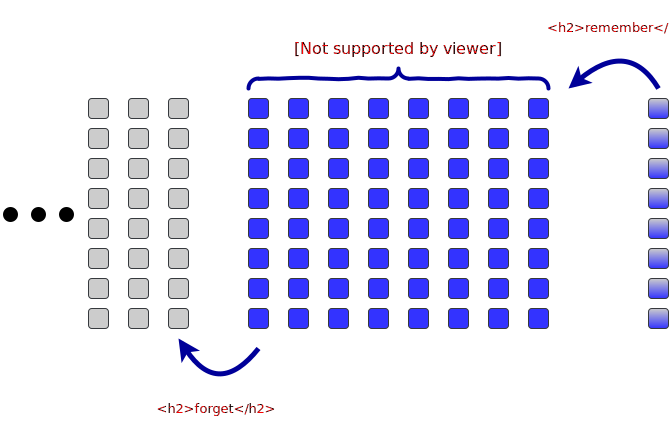
\includegraphics[width=0.85\textwidth]{pool}
	\caption[The exemplar pool]
		{A new exemplar is added to the feature's pool when encountered.
		Old exemplars are removed when the pool is full.
		Exemplars currently in the pool are taken into account when the realization of the feature is determined.
		Each dimension of an exemplar represents a property of the feature it is associated with.}
	\label{fig:exemplar_pool}
\end{figure}
%
This step represents the mental phonetic storage of a speaker, here referred to as a \emph{pool} for a computer-based interlocutor.
The input to it is a feature's exemplar that passed the filtering step and its output is used for updating the feature's representation.
An implementation of such exemplar pool is shown in \cref{subsubsec:collecting_exemplars}.

After an instance of a feature is detected and validated, it needs to be registered as an exemplar of the feature it is associated with.
This stands in parallel to the way such exemplars (and in other contexts also words, meanings, etc.) are mentally stored in the human's short and long term memories.
These accumulated exemplars of a feature determine how a speaker processes it and shape its production when used in speech.
One of the complexities of modeling such internal representation is the interleaving influences of both long-term and short-term memory.
As this pipeline aims to describe convergence occurring within the scope of a single, isolated interaction (even if a long one), only the storage of exemplars is explicitly addressed in it.
However, long-term effects can be implicitly achieved by retaining values between interactions.
To represent short-term memory of feature exemplars, a model must define how and when new exemplars are added, stored, and removed.
\cref{fig:exemplar_pool} gives a schematic overview of such pooling model (and cf.\ the related parameters in \cref{tab:comp_model_parameters}).
In this form, each exemplar is a vector with dimensions standing for its properties, based on the feature it is associated with (e.g., formant values for vowel quality features, pitch changes for intonation-related features, etc.).
Each feature has its own exemplar pool to which newly encountered exemplars are \enquote{memorized}, i.e., added.
This pool is structured as a queue as a very rough, high-level representation of the short-term memory of this feature.
The size of the pool can be defined by a parameter (see \cref{sec:parameters}).
If the pool is already at full capacity when a new exemplar is added, the oldest exemplar will be \enquote{forgotten}, i.e., removed from the feature's pool.
Ultimately, a pool of a feature can be used to determine which exemplars are still affecting the speaker's mental state of a feature.
As the order of the added exemplars is kept, it can be taken into account as well when determining each exemplar's weight, just like recent turns are more likely to impact the current utterance it as ones that occurred at the beginning.

\subsection{Update}
\label{subsec:update}

This step incorporates the process of changing the mental state of a feature based on its accumulated exemplars.
The input to it is the current state of a feature and it outputs a new value for it.

The core of the accommodation process is the actual change in a feature's state.
Many factors may influence this process, both internal and external to the speaker.
The two main considerations in this step is one of each, namely the desired accommodation behavior and the exemplars collected from the user(s) speech input.
The latter is covered by the \enquote{collect} step, and the former is defined using adjustable parameters that correspond to accommodation properties in humans.
For example, how prone is the speaker to be influenced by external others' speech and how easily should the change triggered.
The sensitivity can be constant, or vary based one, e.g., how close the speakers are to each other to begin with.
A trigger might be exemplar-based, i.e., after a certain number of new exemplars were added, or time-based, i.e., every time a certain amount of turns had passed.
\Cref{tab:comp_model_parameters} provides more details about these parameters.
Another means to shape the behavior is the way the new state is computed based on the exemplars.
For example, the computations may make newer exemplars influence the change more.
Moreover, the general accommodation tendency is defined in this step, e.g., converging or diverging from the user's speech, which is determined, among others, by the application.
A \ac{capt} system would probably not aim to align its speech to the user's, but rather diverge from it as a way to present the corrections.
This computation can use simple mathematical operations (as demonstrated in \cref{subsubsec:calculating_changed_value}) or more involved data-driven statistical methods (as the one in \cref{chap:statistical_model}).

\subsection{Assign}
\label{subsec:assign}

This step mediates between the new state of a feature to its use in the system's speech output.
The input to it is the newly calculated state of a feature and it outputs a potentially altered of this state to be used by the \ac{tts} component.

This final step of the pipeline is responsible for assigning the features' representations to the speech production of the system, i.e., as additional input to he \ac{tts} of the system.
For a \ac{tts} module that can directly control the speech output (as part of the model itself or on the outputted waveform),
\putref{refer to chapters with this is discusses when they exist}
The additional information can be used to manipulate the target features in a way that expresses the accommodative behavior of the system.
This closes a circle of feature pronounced by the user and detected by the \ac{asr} component and are now taken into account by the system when speaking back.
Since that means the user will now hear some vocal characteristics that are based on their own speech, it is important to avoid a situation where the user feels imitated -- or even mocked - by the systems.
To that end, this step introduces a limitation mechanism that limits the values given to the \ac{tts} component.
If desired, the values are re-evaluated if some threshold is bypassed (see \cref{eq:new_value}), to avoid such imitation from the system's side.
This mechanism also helps to prevent too extreme values from going the other way.
For example, a \ac{capt} system might demotivate or frustrate the user if its speech is consistently considerably different.
From a human's perspective, this step corresponds to the natural degree to which a speaker would change the realization of a feature.
As shown in \cref{chap:shadowing_experiment_with_natural_and_synthetic_voices,chap:speech_variations_in_hhci}, this varies from feature to feature, and hence this parameter is set for each feature individually (see \cref{tab:comp_model_parameters}).
It is also important that the features are distinguishable and clearly defined by the pipeline, so that the specific modification in the system's speech output can be properly applied in -- and only in -- the correct places, as illustrated in \cref{fig:adapted_synthesis_output}.
%
\begin{figure}
	\centering
	\includegraphics[width=0.85\textwidth]{synthesis}
	\caption
	[Manipulated features on a synthesized waveform]
	{An illustration of a manipulated output audio waveform.
		Each colored pin marks a phonetic features captured and processed by the pipeline.}
	\label{fig:adapted_synthesis_output}
\end{figure}

\section{Parameters}
\label{sec:parameters}

To allow degrees of freedom within the computational model described in \cref{chap:computational_model}, some parameters need to be introduced.
These parameters are the connecting link between the theoretical, schematic model and the implementation of the module as part of an \acs{sds} (see \cref{chap:convergence_module_for_sdss}).
They are also the key for experimentation with the model in various scenarios on the look for the best configurations in different situations.

As shown in \cref{sec:convergence_to_natural_and_synthetic_stimuli}, not all participant showed the same \textit{sensitivity} toward changes in the stimuli in general.
Here sensitivity refers to the degree of adaptation toward a stimulus.
In addition, when one does converge, the sensitivity to changes (i.e.~the \enquote{amount of differentiation}) toward a single stimulus might differ.
In the model, these two aspects were combined into one parameter -- \textit{convergence rate}.
\todo{write a sentence that this rate is a balance between current and new style. put equation}
For simulating the case where a participant does not converge at all, this rate can be set to zero.
In that case the model will ignore the other interlocutor's speech and stick to the current speech style.
Another variation found among the participants was the overall convergence degree toward the stimuli.
In other words, where would the convergence process stop.
This is simulated by the parameters \textit{convergence limit}, which defines the maximally allowed degree of similarity between the interlocutors.
The value of this parameter is between zero and one.
When set to 1.0 (\SI{100}{\percent}), the model is allowed to change up to \SI{100}{\percent} toward the other interlocutor; when set to 0.8, up to \SI{80}{\percent}, and so on.
The parameter is used to control that the model does not simply imitate the user's input, which might happen especially with high convergence rate.
By limiting the change, the convergence process is more gradual and restrained.

However, parameters simulating the actual change are not enough.
To properly model an interlocutor, some individual aspect that are not directly related to the speech output are required as well.

The convergence target depends on the recent instances of the variable feature (or \textit{exemplars}).
How many exemplars are taken into account when the feature's mental representation is updated depends on the interlocutor's short memory capacity.
Working memory is a complex mechanism
\review{reference for modeling working memory?}
.
It is modeled in a very simplified manner here, namely by the number of exemplars the interlocutor currently remembers on a first-in-first-out basis, i.e.~the \textit{exemplar pool size}.
An exemplar is modeled as a vector with cardinality $n$, where $n$ is the number of dimensions the feature has (e.g.~the number of measured formants for a vowel-quality feature).
Whenever an instance of the feature is encountered, a new exemplar is added to the pool.
If the pool is already in full capacity, the oldest exemplar is forgotten by the speaker (deleted in the model) (see \cref{fig:exemplar_pool}).

Individuals may also have different general \textit{tendency} to converge toward other interlocutors.
Here tendency refers to the likelihood to adapt to the stimuli presented to them.
This likelihood is modeled not probabilistically, but by an \textit{update frequency}.
After an exemplar is added to a feature's pool, an update of the feature's value may be triggered.
Whether and how often this happens is determined by the \textit{update frequency}.
If set to 1, an update will occur every time an exemplar is added; if set to 2, every other exemplar, and so on.
When set to 0, however, updates will only take place when explicitly requested.
This can be useful when, for example, all features are to be updated at the same time, regardless of how many exemplars have been accumulated for each feature.
Increasing the update interval means that each new pool value will be affected by more new exemplars, which, depending on the calculation method used (see below), might result in a smoother converging process.
Additionally, a longer update interval also means that convergence will generally take longer, since the model's features are not being updated as frequently.

Though not only the frequency in which the update occurs plays a roll in the process, but also the manner in which it is being updated.
This manner is determined by the \textit{calculation method} used.
Since the features in the model are represented by vectors, any function that takes a vector as input and outputs another as output would do.
\todo{explain that first we need to transform the matrix!}

After transforming the matrix, the model has a representation of each feature as a vector where each dimension is a single value of a 
One option is to use a fixed function on each of the dimensions to create a vector with new values.
This function could be, for example, simple average or decaying average.
Such functions are easy to understand and follow, and can describe relatively simple mechanics of how each stimulus contributes to the overall change, since each value is calculated sequentially but independently of the other.

Each feature can use a different calculation method.
Which method to use is up to the user of the system, as there might be acoustic or psycholinguistic constrains to take into account, based on the settings the system is used in (experimental, exploratory, data collection, etc.)

% calculation method -- make sure you directly lead to it from the update step

\todo{put equations where appropriate}

\begin{landscape}
	\begin{table}[tb]
		\centering
		\caption[Summary of computational model's parameters]{Computational model's parameters in their order of use.}
		\label{tab:comp_model_parameters}
		\begin{tabulary}{\linewidth}{lLL}
			\toprule
			\multicolumn{1}{c}{\textbf{Parameter}} 		& \multicolumn{1}{c}{\textbf{Description}} 					& \multicolumn{1}{c}{\textbf{Value}} \\
			\textit{target phoneme*} 					& the phoneme that triggers the feature 					& phoneme symbol\\
			\textit{phonetic context*} 					& the environment in which the phoneme is accepted 			& regex of phoneme symbols\\
			\textit{allowed range*} 					& the value range in which new instances are accepted 		& numeric, depending on feature\\
			\textit{exemplar pool size} 				& maximum number of exemplars in memory 					& integer, $> 0$\\
			\textit{update frequency} 					& how frequently a feature's value is recalculated 			& integer, $\geq 0$ \\
			\textit{calculation method*} 				& the manner in which the pool value is calculated 			& one of supported methods\\
			\textit{convergence rate} 					& weight given to the pool value 							& float, typically $> 0$ and $< 1$\\
			\textit{convergence limit*}  				& the maximum degree of convergence allowed for a feature 	& float, $> 0$ and $< 1$ \\	
			\bottomrule
		\end{tabulary}
		\flushleft{\footnotesize \emph{* denotes parameters that are defined individually for each feature}}
	\end{table}
\end{landscape}


The model's parameters are summarized in \cref{tab:comp_model_parameters}
With these criteria in mind, a computational model with several parameters wad developed.
This model, described in detail in \citet{Raveh2017Interspeech}, includes these parameters and a few others, and its purpose is to generate different convergence behaviors.

% briefly also mention target phoneme and phonetic context
